% !TeX spellcheck = cs_CZ
%{\tikzset{external/prefix={tikz/FYZI/}}
% \tikzset{external/figure name/.add={ch30_}{}}
%=========================== Kapitola: Difrakce ===================================================
\chapter{Difrakce}\label{fyz:IchapXXX}
\minitoc
  \section{Výsledná amplituda n stejných oscilátorů}\label{fyz:IchapXXXsecI}
    Tato kapitola je přímým pokračováním kapitoly předcházející, i když název se změnil z 
    „interference“ na „difrakci“. Zatím se nikomu nepodařilo uspokojivě definovat rozdíl mezi 
    interferencí a difrakcí. Je to otázka konvence, není mezi nimi nějaký důležitý fyzikální 
    rozdíl. Zhruba je můžeme rozlišit tak, že interferuje-li jen několik zdrojů, například dva, 
    výsledek nazýváme interferencí a je-li zdrojů mnoho, častěji se používá výraz \emph{difrakce}. 
    Nebudeme se proto znepokojovat, zda jde o interferenci nebo difrakci, ale ihned budeme 
    pokračovat v tématu předešlé kapitoly.
    
    Budeme se zabývat \(n\) stejně od sebe vzdálenými oscilátory se stejnými amplitudami, ale 
    různými fázemi, a to buď proto, že kmitají s různými fázemi nebo proto, že na ně hledíme pod 
    takovým úhlem, že sdochází k časovému zpoždění. Z jednoho nebo druhého důvodu musíme sčítat 
    něco jako
    \begin{align}\label{fyz:eq316}
      R = A\big[\cos\omega t &+ \cos(\omega t +  \varphi) +
                              + \cos(\omega t + 2\varphi) + \ldots \nonumber  \\
                      \ldots &+ \cos(\omega t + (n-1)\varphi)\big]
    \end{align}
    kde \(\varphi\) je \emph{fázový rozdíl mezi sousedními oscilátory při pohledu z daného směru}. 
    Přitom platí \(\varphi = \alpha + 2\pi d\sin\vartheta/\lambda\).

    \begin{figure}[ht!] %\ref{fyz:fig249}
      \centering
      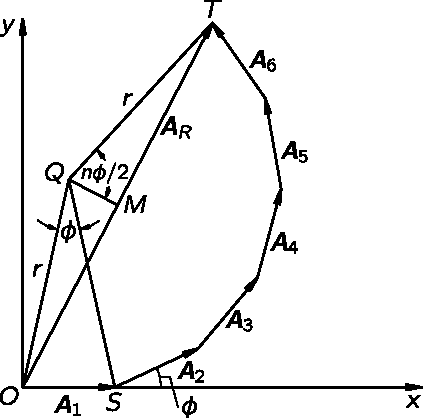
\includegraphics[width=0.8\linewidth]{fyz_fig249.pdf}
      \caption{Výsledná amplituda pro \(n = 6\) rovnoměrně od sebe vzdálených oscilátorů s fázovým 
               rozdílem \(\varphi\) mezi sousednimi oscilátory
               (\cite[s.~392]{Feynman01})}
      \label{fyz:fig249}
    \end{figure}
    
    Nyní musíme sečíst všechny členy. Uděláme to geometricky. První má délku \(A\) a má nulovou 
    fázi. Druhý má také délku \(A\), ale fázi má \(\varphi\). Další má opět délku \(A\) a fázi
    \(2\varphi\) atd. Je jasně vidět, že jde jakoby o pohyb podél \(n\) stran pravidelného 
    mnohoúhelníka (obr. \ref{fyz:fig249}). Jeho vrcholy leží ovšem na kružnici a výslednou 
    amplitudu snadno najdeme, určíme-li poloměr této kružnice.
    
    Předpokládejme, že bod \(Q\) je středem kružnice. Pak úhel \(OQS\) je roven fázi \(\varphi\). 
    (To proto, že poloměr \(QS\) svírá s \(A_2\), stejný úhel jako svírá poloměr \(QO\) s \(A_1\).) 
    Pro poloměr \(r\) pak musí platit
    \begin{equation}\label{fyz:eq317}
      A = 2r\sin\frac{\varphi}{2},
    \end{equation}
    z čehož lze určit \(r\). Velký úhel \(OQT\) je roven \(n\varphi\), takže platí
    \begin{equation}\label{fyz:eq318}
      A_R = 2r\sin\frac{n\varphi}{2}.
    \end{equation}
    Z těchto dvou vztahů vyloučíme \(r\) a dostaneme 
    \begin{equation}\label{fyz:eq319}
      A_R = A\dfrac{\sin\frac{n\varphi}{2}}{\sin\frac{\varphi}{2}}.
    \end{equation}
    Výsledná intenzita je proto
    \begin{equation}\label{fyz:eq320}
      I = I_0\dfrac{\sin^2\frac{n\varphi}{2}}{\sin2\frac{\varphi}{2}}.
    \end{equation}
    Proveďme analýzu tohoto výrazu a podívejme se na některé jeho důsledky. Začneme zkouškou pro 
    \(n = 1\) a správně dostaneme \(I = I_0\). Pro \(n = 2\) můžeme napsat 
    \begin{equation*}
      \sin\varphi = -2\sin\frac{\varphi}{2}\cos\frac{\varphi}{2}
    \end{equation*}
    a máme
    \begin{equation*}
      A_R = 2A\cos\frac{\pi}{2}.
    \end{equation*}
    což souhlasí s (\ref{fyz:eq312}).
    
    Původní myšlenka, proč jsme začali skládat více zdrojů, byla ta, že v jednom směru snad získáme 
    větší intenzitu než v ostatních směrech, že přilehlá maxima, jež bychom měli při dvou zdrojích, 
    budou potlačena. Abychom viděli tento efekt, nakreslíme graf křivky, kterou dostaneme z 
    (\ref{fyz:fig251}) pro velmi velké \(n\) v oblasti blízko (\(\varphi = 0\). Pro \(\varphi\) 
    rovnající se \(0\), máme \(0/0\), ale pro \(\varphi\) infinitezimálně malé je poměr druhých 
    mocnin sinů roven prostě \(n^2\), neboť sinus úhlu je tehdy roven přibližně samotnému úhlu. 
    Intenzita v maximu křivky je proto rovna \(n^2\)-násobku intenzity jednoho oscilátoru.
     
    To lze snadno pochopit, neboť jsou-li všechny oscilátory ve fázi, jejich fázové rozdíly vymizí 
    a všech \(n\) oscilátorů přispívá k výsledné amplitudě stejně, takže amplitudaje \(n\)-krát 
    větší a intenzita je \(n^2\)-krát silnější.
    
    S narůstáním fáze \(\varphi\) se poměr obou sinů začíná zmenšovat a poprvé dosáhne nuly, když 
    \(n\varphi/2 = \pi\), neboť \(\sin\pi = 0\). Jinak řečeno \(\varphi = 2\pi/n\) odpovídá prvnímu 
    minimu křivky (obr. \ref{fyz:fig250}). Chceme-li to vyjádřit pomocí šipek jako na obr. 
    \ref{fyz:fig249}, první minimum se vyskytne tehdy, když se šipky vrátí do počátečního bodu. 
    Znamená to, že celkový úhel složený z příspěvků pootočení jednotlivých šipek, celkový rozdíl 
    fází mezi prvním a posledním oscilátorem, musí být roven \(2\pi\), aby se kružnice uzavřela.

    \begin{figure}[ht!] %\ref{fyz:fig250}
      \centering
      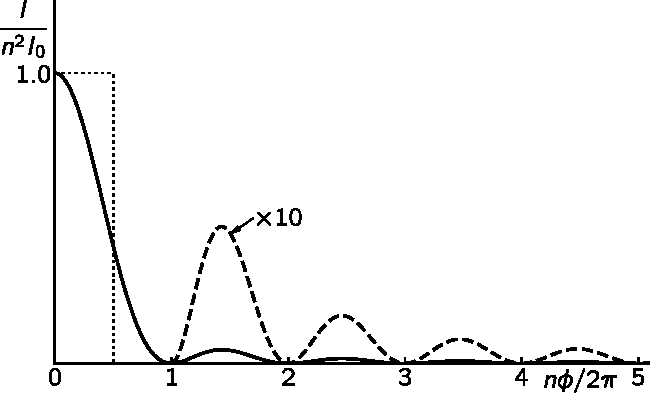
\includegraphics[width=0.8\linewidth]{fyz_fig250.pdf}
      \caption{Intenzita velkého počtu stejně silných oscilátorů jako funkce fázového rozdílu
               (\cite[s.~393]{Feynman01})}
      \label{fyz:fig250}
    \end{figure}
    
    Nyní přejděme k dalšímu maximu, o němž se chceme přesvědčit, zda je opravdu mnohem menší než 
    první maximum, jak doufáme. Nepůjdeme přesně do maxima, neboť jak čitatel tak i jmenovatel 
    (\ref{fyz:eq320}) se mění, avšak \(\sin\varphi/2\) se mění dost pomalu ve srovnání se \(\sin 
    n\varphi/2\) pro velké \(n\), takže když \(\sin n\varphi/2 = 1\), budeme velmi blízko maxima. 
    Toto další maximum nastane, když \(n(\varphi/2) = 3/2\pi\) nebo \(\varphi = 3\pi/n\). To 
    odpovídá tomu, že šipky oběhnou jednu a půl kružnice. Dosazením za \(\varphi = 3\pi/2n\) do 
    našeho vztahu pro velikost druhého maxima máme v čitateli \(\sin^23\pi/2 = 1\) (tak jsme 
    vybrali úhel \(\varphi\)) a ve jmenovateli máme \(\sin^23\pi/2n\). Pro dostatečně velké \(n\) 
    je to velmi malý úhel a sinus je pak roven argumentu, takže pro všechny praktické výpočty 
    můžeme položit \(\sin3\pi/2n = 3\pi/2n\). Zjistili jsme, že intenzita tohoto maxima je \(I = 
    I_04η^2/9\pi^2\). Maximální intenzita byla rovna \(n2I_0\), takže máme \(4/9\pi^2\) násobek 
    intenzity, což je \num{0.047}, tedy méně než 5 \% z maximální intenzity! Samozřejmě, že 
    dál se nacházejí další klesající maxima, takže máme velmi ostré centrální maximum s velmi 
    slabými vedlejšími maximy po stranách. Lze dokázat, že plocha ohraničená křivkou včetně malých 
    maxim je rovna \(2\pi nI_0\), neboli dvojnásobku plochy čárkovaného obdélníku na obr. 
    \ref{fyz:fig250}.

    \begin{figure}[ht!] %\ref{fyz:fig251}
      \centering
      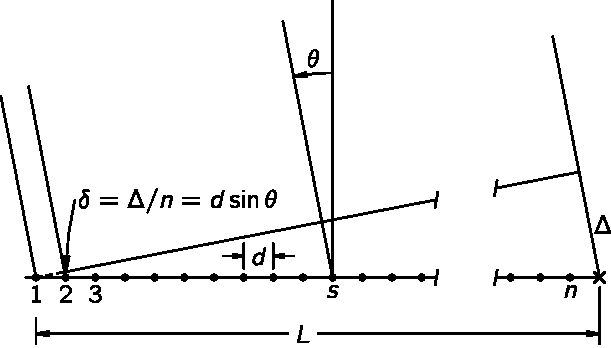
\includegraphics[width=0.9\linewidth]{fyz_fig251.pdf}
      \caption{\(n\) stejných lineárně uspořádaných oscilátorů s fázemi \(\alpha_s = s\alpha\)
               (\cite[s.~394]{Feynman01})}
      \label{fyz:fig251}
    \end{figure}

    Dále se věnujme úvaze o možných aplikacích rovnice (\ref{fyz:eq320}) za různých podmínek a 
    pokusme se pochopit, oč tu jde. Nechť jsou všechny naše zdroje na přímce, jak je to znázorněno 
    na obr. \ref{fyz:fig251}. Dohromady jejich \(n\), všechny jsou od sebe ve vzdálenosti \(d\) a 
    předpokládejme, že relativní fáze mezi sousedními oscilátory je \(\alpha\). Pozorujeme-li je ve 
    směru vytvářejícím s kolmicí úhel \(\vartheta\), je zde ještě dodatečný fázový rozdíl 
    \((2\pi/\lambda)d\sin\vartheta\), způsobený časovým zpožděním mezi sousedy, jak jsme již 
    říkali. Takže:
    \begin{equation}\label{fyz:eq321}
      \varphi = \alpha + \frac{2\pi d}{\lambda}\sin\vartheta = \alpha + kd\sin\vartheta.
    \end{equation}
    
    Nejprve se podíváme na situaci, kdy \(\alpha = 0\), tj. když jsou všechny oscilátory ve fázi a 
    chceme vědět, jak se mění intenzita jako funkce úhlu \(\vartheta\). Stačí nám prostě dosadit 
    \(\varphi = kd\sin\vartheta\) do vztahu (\ref{fyz:eq320}) a podívat se, co se stane. Máme zde 
    především maximum pro \(\varphi=0\). Znamená to, žejsou-li všechny oscilátory ve fázi, ve směru 
    \(\vartheta = 0\) je velká intenzita. Zajímavá je také otázka, kde je první minimum? Nastane 
    pro \(\varphi = 2\pi/n\), takže první minimum má křivka, když platí 
    \begin{align}
      \frac{2\pi d}{\lambda}\sin\vartheta = \frac{2\pi}{n}. \nonumber \\
      \shortintertext{úpravě máme}  
      nd\sin\vartheta = \lambda.                            \label{fyz:eq322}
    \end{align}

    Pokusme se fyzikálně pochopit, proč dostáváme minimum v tomto směru. Součin \(nd\) je celková 
    délka řetězce \(L\). Z pohledu na obr. \ref{fyz:fig251} vidíme, že platí \(nd\sin\vartheta = L 
    \sin\vartheta = \Delta\).
    
    Vztah (\ref{fyz:eq322}) říká, že když je \(\Delta\) rovno \emph{jedné vlnové délce}, dostaneme 
    minimum. Proč nastane minimum, když platí \(\Delta = \lambda\)? Proto, že fáze příspěvků od 
    různých oscilátorů jsou rozděleny rovnoměrně v intervalu od \ang{0} do \ang{360}. Šipky na obr. 
    \ref{fyz:fig249} vytvářejí úplnou kružnici - sčítáme stejné vektory směřující na všechny strany 
    a takový součet je roven nule. Takže, když máme úhel, pro který \(\Delta = \lambda\), máme 
    minimum. To je první minimum.
    
    Vztah (\ref{fyz:eq320}) se vyznačuje další zajímavou vlastností a to tou, že se vůbec nezmění, 
    když se \(\varphi\) zvětší o jakýkoliv násobek \(2\pi\). Takže pro (\(\varphi = 2\pi, 4\pi, 
    6\pi\) atd. dostaneme další silná maxima. Při každém velkém maximu se opakuje průběh znázorněný 
    na obr. \ref{fyz:fig250}. Můžeme si klást otázku, jaké geometrické uspořádání dává další 
    maxima? Podmínkouje, aby \(\varphi=2\pi m\), kde \(m\)e celé číslo, tj. aby platilo
    \begin{align}
      \frac{2\pi d}{\lambda}\sin\vartheta = 2\pi m.         \nonumber \\
      \shortintertext{ Odtud po dělení \(2\pi\) dostaneme}  
      d\sin\vartheta = m\lambda.                            \label{fyz:eq323}
    \end{align}

    To vypadá jako další vztah (\ref{fyz:eq322}). Ale není to tak, ten byl 
    \begin{equation*}
      nd\sin\vartheta = \lambda.
    \end{equation*}
    
    Rozdíl je v tom, že tady se musíme dívat na \emph{jednotlivé zdroje} a když platí 
    \(d\sin\vartheta = m\lambda\), znamená to, že úhel \(\vartheta\) je takový, že \(\delta= 
    m\lambda\) (viz obr. \ref{fyz:fig251}). Jinak řečeno, každý zdroj nyní přispívá určitým dílem a 
    následující zdroje jsou fázově posunuty o celý násobek \ang{360}, a proto přispívají 
    \emph{ve fázi}, fázový posun o \ang{360} znamená totéž jako být ve fázi. Všechny zdroje 
    přispívají stejnou fází a vytvářejí stejně dobré maximum, jaké bylo pro \(m = 0\), o němž jsme 
    mluvili předtím. Vedlejší maxima a celkový průběh intenzity mají stejný průběh, jako to bylo v 
    blízkosti \(\varphi = 0\), s týmiž minimy po obou stranách atd. Proto takový řetězec zdrojů 
    vysílá paprsky v různých směrech a každý z nich má silné centrální maximum a určitý počet 
    slabých „vedlejších laloků“. Silným paprskům se také říká paprsky nultého řádu, paprsek prvního 
    řádu atd. a to podle hodnoty \(m\), která se nazývá \(řád\) paprsku.
    
    Je třeba upozornit na skutečnost, že je-li \(d\) menší než \(\lambda\), nemůže mít rovnice 
    (\ref{fyz:eq323}) jiné řešení, než pro \(m = 0\), takže když je vzdálenost mezi sousedními 
    zdroji velmi malá, existuje jen jeden paprsek - paprsek nultého řádu soustředěný ve směru 
    \(\vartheta = 0\); a samozřejmě i v opačném směru. Abychom dostali dodatečná velká maxima, musí 
    být vzdálenost \(d\) větší než jedna vlnová délka.
    
  \section{Difrakční mřížka}\label{fyz:IchapXXXsecII}
    V technické praxi s anténami a dráty lze vše upravit tak, že fáze všech malých oscilátorů nebo 
    antén jsou stejné. Otázkou je, zda a jak toho můžeme dosáhnout se světlem. Dnes ještě 
    nedokážeme zkonstruovat malé radiostanice s optickou frekvencí, pospojovat je nekonečně malými 
    drátky a budit je všechny se stejnou fází. Ale lze toho dosáhnout jinak.
    
    Předpokládejme, že bychom měli mnoho rovnoběžných drátů rovnoměrně rozložených se vzdáleností 
    \(d\) a nějaký velmi vzdálený zdroj kmitající s rádiovou frekvencí a budící elektromagnetické 
    pole, jež dopadá na všechny dráty se stejnou fází (tj. tak daleko, že časové zpoždění je pro 
    všechny dráty stejné). Bylo by možné vymyslet případ, kdy jsou dráty na zakřivené ploše, ale 
    mluvme jen o rovině. Vnější elektrické pole bude nutit elektrony v každém drátu, aby kmitaly 
    nahoru a dolů. Takže pole, přicházející od původního zdroje, bude pohánět elektrony nahoru a 
    dolů, a tak vzniknou nové generátory. Tomuto jevu se říká \emph{rozptyl}: světelná vlna z 
    nějakého zdroje může indukovat pohyb elektronů v nějakém materiálu a tyto pohyby generují své 
    vlastní vlny. Je tedy třeba rozložit mnoho stejně vzdálených drátů, vybudit je vzdáleným 
    zdrojem elektromagnetického pole a máme, co jsme chtěli, vše bez mnoha speciálních zapojení. 
    Je-li dopadající vlna ve směru normály, všechny fáze budou stejné a budeme mít přesně to, o čem 
    jsme mluvili. Takže, jsou-li vzdálenosti mezi dráty větší než vlnová délka, dostaneme velkou 
    intenzitu rozptylu ve směru normály a v dalších směrech daných vztahem (\ref{fyz:eq323}).
    
    \emph{Obdobně to můžeme provést i se světlem}. Místo drátů použijeme kousek plochého skla a 
    uděláme do něho vrypy, takové, že každý vryp rozptyluje světlo trochu jinak než zbytek skla. 
    Posvítíme-li potom na sklo, každý vryp bude představovat nějaký zdroj, a budou-li velmi blízko 
    vedle sebe, ne však blíže než vlnová délka (což je i technicky téměř nemožné), budeme očekávat 
    zázračný jev: Světlo nejen, že bude procházet sklem, ale vznikne i silný paprsek pod určitým 
    úhlem, v závislosti na vzdálenosti mezi vrypy. Takové objekty byly skutečně vyrobeny a běžně se 
    používají - nazývají se \textbf{difrakční mřížky}.
    
    Jedna z forem takové difrakční mřížky není opravdu nic jiného než jednoduchá rovinná tabulka 
    průhledného a bezbarvého skla, do níž jsou vyryty vrypy. Na jednom milimetru bývá často i 
    několik set rovnoměrně rozložených vrypů velmi pečlivě uspořádaných ve stejných vzdálenostech. 
    Účinek takové mřížky je možné dobře vidět pomocí projektoru, jenž na plátno vrhá úzký 
    vertikální proužek světla (obraz nějaké úzké štěrbiny). Vložíme-li do takového paprsku 
    difrakční mřížku s vrypy otočenými vertikálně, vidíme, že proužek světla na plátně zůstal a 
    navíc máme pokaždé straně další výraznou světelnou stopu, která je \emph{barevná}. Odpovídá 
    obrazu štěrbiny roztaženému ve velkém rozsahu úhlů, neboť úhel \(\vartheta\) ve vztahu 
    (\ref{fyz:eq323}) závisí navlnové délce \(\lambda\) a jak víme, světlu různých barev přísluší 
    různé frekvence, a tedy i různé vlnové délky.
    
    Největší viditelná vlnová délka odpovídá červené barvě a protože \(dsin\vartheta= \lambda\) je 
    \(\vartheta\) pro červenou barvu největší. Na plátně opravdu vidíme, že červená je posunuta od 
    středu o největší úhel! Na druhé straně by se také měl nacházet takový paprsek a opravdu ho i 
    vidíme. Dále, vztah (\ref{fyz:eq323}) může mít i další řešení pro \(m = 2\). Skutečně neurčitě 
    vidíme, že tam něco je - velmi slabý paprsek - a za ním jsou dokonce vidět i další paprsky.
    
    Právě jsme dokazovali, že všechny tyto paprsky mají mít stejnou intenzitu, ale zjistili jsme, 
    že ji nemají a dokonce ani první paprsek vpravo a vlevoji nemají stejnou! Důvodem je to, že 
    mřížka byla pečlivě vyrobena, aby se chovala právě tak. Kdyby se mřížka skládala z velmi 
    jemných vrypů nepatrné šířky, rozložených rovnoměrně, intenzity všech paprsků by byly skutečně 
    stejné. Ale i v nejjednodušším případě bychom mohli uvažovat uspořádání dvojic antén, z nichž 
    každá má určitou intenzitu a nějakou relativní fázi. V takovém případě můžeme získat paprsky, 
    které se v různých řádech liší intenzitou. Mřížka se často nezískává z malých symetrických 
    vrypů, ale pomocí rýh, jež mají pilovitý profil. Důmyslným uspořádáním těchto zubů lze 
    dosáhnout toho, že víc světla jde do paprsků jednoho daného řádu spektra než do ostatních. V 
    praxi je výhodné, když mřížka dává paprsky s maximální intenzitou v některém řádu. Může se 
    zdát, že je to příliš komplikovaný případ, abychom zde o něm mluvili, ale je to opravdu velmi 
    důmyslná věc, neboť mřížka se tak stává užitečnější.
    
    \begin{figure}[ht!] %\ref{fyz:fig252}
      \centering
      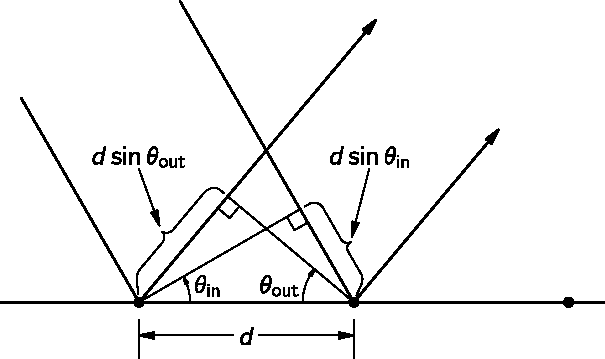
\includegraphics[width=0.8\linewidth]{fyz_fig252.pdf}
      \caption{Dráhový rozdíl paprsků rozptylovaných sousedními rýhami difrakční mřížky je 
               \(d\sin\vartheta_2 - d\sin\vartheta_1\)
               (\cite[s.~396]{Feynman01})}
      \label{fyz:fig252}
    \end{figure}
    
    Dosud jsme se zabývali případem, kdy všechny zdroje byly ve fázi. Máme však vztah pro úhel 
    \(\varphi\) pro případ, liší-li se sousední fáze o úhel \(\alpha\). Vyžaduje to takové zapojení 
    antén, aby mezi nimi byl malý fázový posun. Můžeme toho dosáhnout i u světla? Ano, a to velmi 
    snadno. Předpokládejme, že světlo přichází z nekonečně vzdáleného zdroje pod určitým úhlem 
    \(\vartheta_1\) a řekněme, že se zajímáme o rozptýlené světlo, jež vychází pod úhlem 
    \(\vartheta_2\). Úhel \(\vartheta_2\), je tentýž úhel \(\vartheta\), který jsme měli předtím 
    a \(\vartheta_1\), sloužíjen k tomu, aby zdroje byly uspořádány s různými fázemi. Světlo 
    přicházející ze vzdáleného budicího zdroje nejprve dosáhne první rýhy, pak další a další atd. s 
    fázovým posunem mezi rýhami, jenž jak vidíme je roven
    
    \begin{equation*}
      \alpha = - \frac{d\sin\vartheta_1}{\lambda}
    \end{equation*}
    Tak máme vztah pro fázový úhel mřížky, u níž světlo dopadá pod různými úhly:
    \begin{equation}\label{fyz:eq324}
      \varphi = \frac{2\pi d}{\lambda}\sin\vartheta_2 - 
                \frac{2\pi d}{\lambda}\sin\vartheta_1.               
    \end{equation}
    
    Pokusme se zjistit, kde za těchto okolností dostaneme silnou intenzitu. Podmínkou pro silné 
    intenzity je, že \(\varphi\) má být rovno celému násobku \(2\pi\). Je tu několik zajímavostí, 
    jichž si musíme všimnout.
    
    Jeden velmi zajímavý případ odpovídá hodnotě \(m = 0\); pro \(d\) menší než \(\lambda\) je to 
    fakticky jediné řešení. Vidíme, že v tomto případě \(\sin\vartheta_2 = \sin\vartheta_1\), což 
    znamená, že vycházející světlo má stejný směr jako světlo, které vybudilo difrakční mřížku. 
    Mohli bychom si myslet, že světlo mřížkou přímo prochází. Ale pozor, my zde mluvíme o 
    \emph{jiném světle}. Světlo, jež prochází přímo, je světlo z původního zdroje. Světlo, o němž 
    mluvíme, je nové světlo vybuzené rozptylem. Vychází nám, že rozptýlené světlo letí ve stejném 
    směru jako původní a může s ním interferovat - jev, jímž se budeme zabývat později.
    
    V tomto případě existuje ještě další možnost. Pro dané \(\vartheta_1\) může být 
    \(\vartheta_2\), rovno \(\pi-\vartheta_1\). A tak nejenže dostáváme paprsek ve stejném směru 
    jako dopadající paprsek, ale i v dalším směru,jenž je takový (uvážíme-li to pozorně), že 
    \emph{úhel dopadu je roven úhlu rozptylu} - tento paprsek nazýváme \emph{odražený paprsek}.
    
    Tak začínáme chápat základní mechanizmus odrazu světla: Dopadající světlo vyvolává pohyby atomů 
    v odražeči a ten vytváří \emph{novou vlnu}. Jedno z řešení pro směr rozptylu (je to jediné 
    řešení pro případ, že vzdálenost rozptylových center je velmi malá v porovnání s vlnovou délkou 
    světla) je, že úhel, pod kterým světlo vychází, je roven úhlu, pod kterým dopadá!
    
    Nyní se podívejme na zvláštní případ, kdy \(d\rightarrow 0\). Mějme kousek skla konečných 
    rozměrů a požadujme, aby se fázový rozdíl mezi sousedními rozptylovými centry blížil k nule. 
    Jinak řečeno, mezi existující „antény“ vkládáme další, takže rozdíly fází se zmenší, přičemž se 
    však celkový fázový rozdíl mezi začátkem a koncem řady nezmění. Podívejme se, co se stane s 
    (\ref{fyz:eq320}), zachováme-li rozdíl fází mezi první a poslední anténou konstantní. (Řekněme, 
    že je roven \(n\varphi = \Phi\)), počet antén necháme narůstat do nekonečna a fázový posun 
    (\(\Phi_2\) každé antény se bude blížit k nule. Nyní pro malé \(\varphi\) platí 
    \(\sin\varphi=\varphi\) a když si vzpomeneme, že \(n^2I_0\) je \(I_m\), maximální intenzita ve 
    středu paprsku, zjistíme, že
    \begin{equation}\label{fyz:eq325}
      I = \frac{4I_m\sin^2\dfrac{\Phi}{2}}{\Phi^2}.
    \end{equation}
    Tento limitní případ je znázorněn na obr. \ref{fyz:fig249}
    
    Za těchto okolností dostáváme stejný obecný obraz jako pro případ konečně vzdálených antén s 
    \(d > \lambda\); všechny vedlejší laloky jsou prakticky stejné, chybějí pouze maxima vyšších 
    řádů. Pro všechna rozptylová centra ve fázi dostáváme maximum ve směru \(\vartheta_2 = 0\) a 
    minimum, je-li vzdálenost \(\Delta\) rovna \(\lambda\) jako v případě konečného \(d\) a \(n\). 
    Takže můžeme analyzovat dokonce i spojité rozdělení rozptylových center nebo oscilátorů, 
    použijeme-li místo sum integrály.
    
    Pro ilustraci si představme dlouhý řetězec oscilátorů s náboji oscilujícími ve směru řetězce 
    jako na obr. \ref{fyz:fig253}. Největší intenzita od takto seřazených antén je ve směru kolmém 
    na směr řetězce. Ve směru nad a pod rovníkovou rovinou je také rozložena část intenzity, ale 
    velmi slabá. Pomocí tohoto výsledku můžeme řešit i složitější situace. Představme si, že máme 
    několik takových řetězců, z nichž každý vytváří paprsek jen v rovině na něho kolmé. Najít, jaká 
    je intenzita paprsků v různých směrech od série dlouhých drátů místo od infinitezimálně 
    krátkých drátů, je týž problém, dokud jsme ve střední rovině kolmé na dráty - příspěvky od 
    jednotlivých vodičů prostě sčítáme. To je důvod, proč jsme naši analýzu malých antén mohli 
    použít i pro mřížku s dlouhými úzkými rýhami. Učinek každé z těchto rýh se projeví jen ve směru 
    na ní kolmém (nikoli ve směru šikmo nahoru nebo dolů), ale protože jsou všechny uspořádány 
    vodorovně, tímto způsobem interferují.

    \begin{figure}[ht!] %\ref{fyz:fig253}
      \centering
      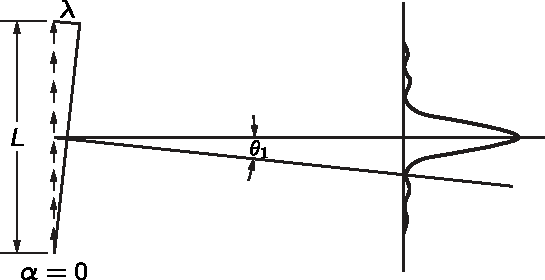
\includegraphics[width=0.9\linewidth]{fyz_fig253.pdf}
      \caption{Průběh intenzity oscilátorů spojitě rozložených na přímce má jedno silné maximum a 
               mnoho slabých bočních,„laloků“
               (\cite[s.~398]{Feynman01})}
      \label{fyz:fig253}
    \end{figure}
    
    Takto bychom mohli vytvořit i složitější situace - rozložením různých rozptylových center podél 
    přímek v rovinách nebo v prostoru. Nejdřív jsme provedli analýzu pro rozptylová centra 
    rozložená na přímce a pak jsme ji rozšířili pro rovnoběžné pásky. To lze provést prostým 
    sčítáním příspěvků jednotlivých oscilátorů. Princip je vždy stejný.
    
  \section{Rozlišovací schopnost mřížky}\label{fyz:IchapXXXsecIII}
    Dostali jsme se tak daleko, že můžeme pochopit celou řadu zajímavých jevů. Například jak by 
    bylo možné využít difrakční mřížku k odlišení vlnových délek. Všimli jsme si, že na plátně bylo 
    rozprostřeno celé spektrum barev, takže difrakční mřížku lze použít jako nástroj k rozložení 
    světla na jeho různé vlnové délky.Jednou ze zajímavých otázek je: Předpokládejme, že máme dva 
    zdroje, jejichž frekvence nebo vlnové délky se liší jen málo; jak malý musí být rozdíl jejich 
    vlnových délek, aby pomocí difrakční mřížky nebylo možné zjistit, že jde o dvě různé vlnové 
    délky? Červenou a modrou vlnovou délku bylo možné jasně rozlišit, ale jak malý by musel být 
    rozdíl vlnových délek, kdyby jedna vlnová délka byla červená a druhá jen trochu červenější? To 
    je vlastnost, jež se nazývá \emph{rozlišovací schopnost} mřížky a jeden možný způsob, jak ji 
    určit, je následující. Předpokládejme, že maximum rozptýleného světla nějaké barvy máme pro 
    paprsek vycházející pod určitým úhlem. Se změnou vlnové délky měníme i fázi \(2\pi 
    d\sin\vartheta/\lambda\), takže maximum nastane pod jiným úhlem. To je důvod, proč červená a 
    modrá jsou odděleny. Jak velká musí být tato změna úhlu, abychom tento rozdíl postřehli? 
    Překrývají-li se obě maxima, je pochopitelné, že je nerozlišíme. Je-li jedno maximum dostatečně 
    daleko od druhého, budeme ho pozorovat jako dvojité. K rozlišení takových dvou blízkých maxim 
    se používá \textbf{Rayleighovo kritérium} (obr. \ref{fyz:fig254}): první minimum od jednoho 
    zdroje musí ležet na maximu od druhého zdroje. Nyní, leží-li jedno minimum na druhém maximu, 
    lze snadno vypočítat, jaký musí být příslušný rozdíl vlnových délek. Nejlépe je to provést 
    geometricky.
    
    \begin{figure}[ht!] %\ref{fyz:fig254}
      \centering
      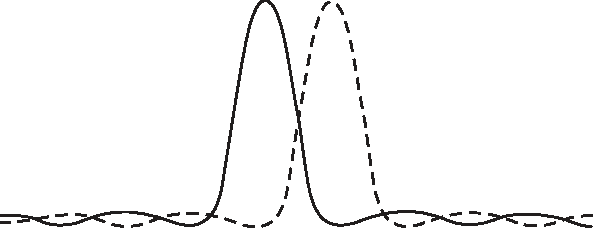
\includegraphics[width=0.7\linewidth]{fyz_fig254.pdf}
      \caption{Znázornění Rayleighova kritéria. Maximum od jednoho zdroje leží na prvním minimu od 
               druhého zdroje.
               (\cite[s.~399]{Feynman01})}
      \label{fyz:fig254}
    \end{figure}
    
    Abychom měli maximum provlnovou délku \(\lambda'\), musí být vzdálenost \(\Delta\) (obr. 
    \ref{fyz:fig251}) rovna \(n\lambda'\) a jde-li o paprsek \(m\)-tého řádu, tak \(mn\lambda'\). 
    Takže
    \begin{equation*}
      \dfrac{2\pi d}{\lambda'}\sin\vartheta =2\pi m 
    \end{equation*}
    
    a \(\Delta\) rovné \(nd\sin\vartheta\), je vlastně \(\lambda‘\) krát \(n\) nebo \(mn\). Chceme, 
    aby druhý paprsek s vlnovou délkou \(\lambda\) měl přitom to úhlu své minimum. To znamená, že 
    chceme, aby \(\Delta\) bylo přesně ojednu vlnovou délku větší než \(mn\lambda\):
    \begin{equation*}
      \Delta = mn\lambda + \lambda = mn\lambda'.
    \end{equation*}
    Když \(\lambda' = \lambda + \Delta\lambda\), platí
    \begin{equation}\label{fyz:eq326}
      \frac{\Delta\lambda}{\lambda} = \frac{1}{mn}.
    \end{equation}
    
    Poměr \(\lambda/\Delta\lambda\) se nazývá rozlišovací schopnost mřížky. Vidíme, že je rovna 
    součinu celkového počtu vrypů mřížky \(n\) a řádu \(m\). Není těžké ukázat, že tento vztah je 
    ekvivalentní vztahu, podle něhož je změna frekvence rovna převrácené hodnotě rozdílu časů 
    náležících dvěma extrémním dráhám, po nichž se pohybují interferující paprsky\footnote{v našem 
    případě \(T=\frac{\Delta}{c} = \frac{mn\lambda}{c}\), kde \(c\) je rychlost světla. Frekvence 
    \(f = \frac{c}{\lambda}\), takže \(\Delta f = \frac{c\Delta\lambda}{\lambda^2}\).}
    \begin{equation*}
      \Delta f =\frac{1}{T}.
    \end{equation*}
    
    Nejlépe je zapamatovat si tento vztah, neboť platí obecně, nejen pro mřížky, ale pro jakýkoliv 
    přístroj, zatímco vztah (\ref{fyz:eq326}) vyjadřuje fakt, že jde o mřížku.
    
  \section{Parabolická anténa}\label{fyz:IchapXXXsecIV}
    Podívejme se na jiný problém spojený s rozlišovací schopností. Souvisí s radioteleskopickou 
    anténou, jaká se používá při určování polohy zdrojů rádiových vln na obloze a jejich úhlové 
    velikosti. Samozřejmě, kdybychom vzali jakoukoli z dříve používaných antén a zachytili signál, 
    nevěděli bychom, odkud přichází. My však chceme vědět, jestli se zdroj nachází na tom nebo na 
    onom místě. Jeden způsob, jak to zjistit, je rozložit celou sérii rovnoměrně vzdálených 
    dipólových antén, například po území Austrálie. Pak zapojíme přívody těchto antén do téhož 
    přijímače a to tak, aby časový posun byl ve všech napájecích linkách stejný. Přijímač tedy 
    přijímá signály od všech dipólů ve fázi a všechny vlny ve fázi sčítá. Co se stane? Nachází-li 
    se zdroj přímo nad anténami v téměř nekonečné vzdálenosti, dopadající rádiové vlny vybudí 
    všechny antény ve fázi, všechny společně napájejí přijímač. 
    
    Dále předpokládejme, že se radiovysílač nachází ve směru, jenž se od svislého směru odchyluje o 
    nějaký malý úhel \(\vartheta\). Různé antény pak přijímají signály s malými fázovými rozdíly, V 
    přijímači se tyto nesfázované signály sčítají a je-li úhel \(\vartheta\) příliš velký, nic 
    neslyšíme. Jak velký může být úhel \(\vartheta\)? Nulový signál dostaneme, když úhel \(\Delta/L 
    =\vartheta\) (obr. \ref{fyz:fig251}) odpovídá fázovému posunu \(2\pi\), tj., když je \(\Delta\) 
    rovno vlnové délce \(\lambda\). Tehdy vektorové příspěvky vytvářejí uzavřený mnohoúhelník s 
    nulovou výslednicí. Nejmenší úhel, který může rozlišit anténa délky \(L\), je \(\vartheta = 
    \lambda/L\). Všimněme si, že směrová citlivost antény je stejná, jak by bylo rozložení 
    intenzity jí vysílaných signálů, kdybychom přijímač vyměnili za vysílač. Máme příklad toho, 
    čemu se říká princip reciprocity. Pro jakékoli seskupení antén, pro jakékoli úhly a podobně 
    obecně platí, že zjistíme-li nejdříve relativní intenzity signálů v různých směrech, při 
    zapojení antény na vysílač, relativní směrová citlivost přijímače se stejně zapojeným systémem 
    antén je stejná jako byla relativní intenzita vysílaných vln. 
    
    Některé rádiové antény jsou zkonstruovány jinak. Místo mnoha dipólů seřazených podél dlouhé 
    přímky a pospojovaných s přijímačem množstvím drátů mohou být seřazeny do tvaru vhodné křivky s 
    přijímačem umístěným na vhodném místě, kde může zachycovat rozptýlené vlny. Tvar takové křivky 
    je možné navrhnout tak, že když rádiové vlny přicházejí přesně shora, rozptýlené vlny dopadnou 
    na přijímač současně (obr. \ref{fyz:fig290}). Takovou křivkou je parabola a nacházíli se zdroj 
    přesně v její ose, dostaneme v jejím ohnisku signál velké intenzity. Rozlišovací schopnost 
    takového přístroje je jasná. Rozestavení antén po parabolické křivce zde není podstatné. Je to 
    jen vhodný způsob, jak dostat všechny signály do jednoho bodu současně a bez připojovacích 
    kabelů. Rozlišovací úhel takového zařízení je stále  \(\vartheta =  \lambda/L\), kde \(L\) je 
    vzdálenost mezi krajními anténami. Tento úhel nezávisí na velikosti mezer mezi anténami, jež 
    mohou býti těsně vedle sebe nebo dokonce mohou tvořit jeden kus kovu. Řeč je samozřejmě o 
    teleskopickém zrcadle a vlastně jsme určili rozlišovací schopnost zrcadlového dalekohledu! 
    Někdy se uvádí, že rozlišovací schopnost je \(\vartheta = \num{1.22}\lambda/L\), kde \(L\) je 
    průměr teleskopu. Důvod, proč to není přesně \(\lambda/L\) je tento: Při odvozování výsledku 
    \(\vartheta = \lambda/L\) jsme předpokládali, že všechny dipóly jsou stejně výkonné, ale 
    teleskop je obyčejně kruhovitý, a proto z jeho okrajů nepřichází tak silný signál, jaký by 
    přicházel od rovinné desky, na níž by byla všude stejná intenzita. Na okrajích využíváme 
    teleskop jen částečně, takže celková intenzita je o něco menší. Chápeme proto, že efektivní 
    průměr je o něco menší než skutečný průměr a to je vyjádřeno faktorem \(1,22\). V každém 
    případě, takové přesné vyjádření vztahu pro rozlišovací schopnost se zdá být příliš 
    přehnané\footnote{ Je to v především proto, že Rayleighovo kritérium je jen hrubý odhad. Říká 
    nám, kdy začíná být obtížné rozlišit obrazy dvou blízkých hvězd. Ve skutečnosti, je-li možno 
    provést dostatečně přesné měření rozložení intenzity v oblasti světelné skvrny vzniklé 
    difrakcí, lze oba zdroje rozlišit i pro to \(\vartheta\) menší než \(\lambda/L\).}.
    
  \section{Barvy tenkých vrstev; krystaly}\label{fyz:IchapXXXsecV}
    Uvedli jsme některé interferenční jevy, které vznikají skládáním různých vln. Existuje však 
    mnoho dalších příkladů interference, a i když zatím ještě nerozumíme podstatě jejího mechanizmu 
    víme už nyní jak k interferenci dochází. Například při dopadu světelné vlny na povrch látky s 
    indexem lomu \(n\), řekněme pod pravým úhlem, se část světla odrazí. Důvod, proč nastává odraz, 
    si rozebereme později. Předpokládejme však, že víme, že část světla se odrazí jak při vstupu 
    tak i výstupu z odrazivého prostředí. Podíváme-li se na odraz světla na tenké vrstvě, vidíme 
    součet dvou vln. Je-li tloušťka vrstvy dostatečně malá, dojde k interferenci těchto dvou vln, 
    konstruktivní nebo destruktivní, v závislosti na znaménkách fází. Může se například stát, že 
    pro červenou barvu dostaneme zesílený odraz, ale pro modrou, jež má jinou vlnovou délku, 
    dostaneme zeslabený odraz v důsledku destruktivní interference, takže vidíme jasný červený 
    odraz. Změníme-li tloušťku, tj. podíváme-li se na jiné místo, kde je vrstva tlustší, může to 
    být naopak - červená se zeslabí, ale ne modrá, takže obraz zdroje je jasně modrý nebo     
    zelený nebo žlutý nebo jiný. Proto při pohledu na tenké vrstvy vidíme barvy a ty se mění, 
    díváme-li se z různých úhlů, neboť již víme, že fázové rozdíly jsou různé pro různé úhly. Tak 
    umíme pochopit mnoho dalších případů, když při různých úhlech vidíme barvy na olejových 
    vrstvách, mýdlových bublinách apod. Princip je však vždy stejný - sčítají se vlny s rozdílnými 
    fázemi. Vzpomeneme i další důležitou aplikaci difrakce. U mřížky jsme viděli na plátně 
    difrakční obrazec. Kdybychom použili monochromatické světlo, nacházelo by se maximum na určitém 
    místě. Byla by tam i další maxima vyšších řádů. Z polohy difrakčních obrazců bychom mohli určit 
    vzdálenost rýh na mřížce, kdybychom znali vlnovou délku světla. Z rozdílů v intenzitě mezi 
    jednotlivými obrazci bychom mohli zjistit profil rýh tvořících mřížku - ať jsou to drátky, 
    pilovité rýhy nebo něco jiného, a to \emph{aniž bychom mřížku viděli} Stejný princip se používá 
    při identifikaci polohy \emph{atomů v krystalech}. Jedinou těžkostí je, že krystal je 
    trojrozměrný útvar - opakující se trojrozměrné uspořádání atomů. K tomu nemůžeme použít 
    obyčejné světlo, ale něco, co má vlnovou délku menší než je vzdálenost mezi atomy, neboť jinak 
    nedostaneme interferenci. Musíme proto použít záření s velmi krátkou vlnovou délkou, tj. 
    rentgenové záření. Osvětlíme-li krystal rentgenovým zářením a všimneme si intenzity odrazu v 
    různých řádech, můžeme určit, jak jsou uspořádány atomy v krystalu, aniž bychom je viděli okem. 
    Tak poznáme uspořádání atomů v různých látkách a to nám umožnilo nakreslit v kapitole 
    \ref{fyz:IchapI} rozložení atomů v krystalu kuchyňské soli apod. Později se k tomu ještě 
    vrátíme, abychom si toto velmi zajímavé téma probrali mnohem podrobněji; zatím se spokojíme s 
    tímto stručným výkladem.
  
  \section{Difrakce na neprůzračné cloně}\label{fyz:IchapXXXsecVI}
    Nyní se dostáváme k velmi pozoruhodné situaci. Předpokládejme, že na jedné straně máme 
    nepropustnou desku s otvory a vedle ní zdroj světla. Chceme zjistit, jaká je intenzita světla 
    na druhé straně. Většina lidí řekne, že světlo svítí otvory a osvětluje druhou stranu. Ukazuje 
    se, že správnou odpověď ve velmi dobrém přiblížení dostaneme, budeme-li předpokládat, že zdroje 
    světla jsou rovnoměrně rozloženy v jednotlivých otvorech a jejich fáze jsou takové jako kdyby 
    tam nepropustná deska nebyla. Samozřejmě, ve skutečnosti v otvorech nejsou žádné zdroje, v 
    tomto případě jsou to vlastně jediná místa, kde zcela určitě nejsou zdroje. Přesto správný 
    difrakční obrazec dostaneme za předpokladu, že otvory jsou jediná místa, kde zdroje jsou - to 
    je dost divné. Vysvětlíme si to později, zatím předpokládejme, že je to tak.
    
    V teorii difrakce se vyskytuje další druh difrakce, který si stručně probereme. V základním 
    kurzu se o něm obvykle nemluví už tak brzy, jak to děláme my, a to jen proto, že ke sčítání 
    malých vektorových příspěvků je třeba použít o něco složitější matematické vzorce. Jinak je to 
    úplně stejné jako to, co jsme dělali dosud. Všechny interferenční jevy jsou stejné, nejde v 
    podstatě o nic náročnějšího, jen situace je tady složitější a zmiňované vektory lze hůře 
    spočítat.

    \begin{figure}[ht!] %\ref{fyz:fig255}
      \centering
      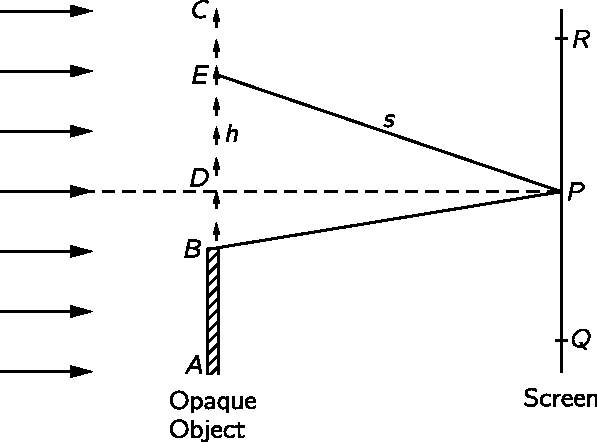
\includegraphics[width=0.8\linewidth]{fyz_fig255.pdf}
      \caption{Vzdálený zdroj světla vrhá na stínítko stín neprůhledného předmětu.
               (\cite[s.~402]{Feynman01})}
      \label{fyz:fig255}
    \end{figure}
    
    Předpokládejme, že světlo letící z nekonečna vrhá stín nějakého předmětu. Obr. \ref{fyz:fig255} 
    znázorňuje stínítko, na které dopadá stín od předmětu \(AB\), přičemž zdroj světla je velmi 
    daleko v porovnání s vlnovou délkou světla. Dalo by se očekávat, že mimo stín bude osvětlení 
    všude jasné a ve stínu bude všude tma. Kdybychom si však znázornili intenzitu jako funkci 
    polohy v blízkosti okraje stínu, viděli bychom, že zpočátku stoupá, pak překročí vrchol a kmitá 
    velmi zvláštním způsobem v blízkosti okraje (obr. 30.9). Podívejme se, proč tomu tak je. 
    Použijeme-li větu, kterou jsme ještě nedokázali, můžeme skutečnou situaci nahradit sérií 
    zdánlivých zdrojů rozložených rovnoměrně v prostoru za objektem AB.


    \begin{figure}[ht!] %\ref{fyz:fig256}
      \centering
      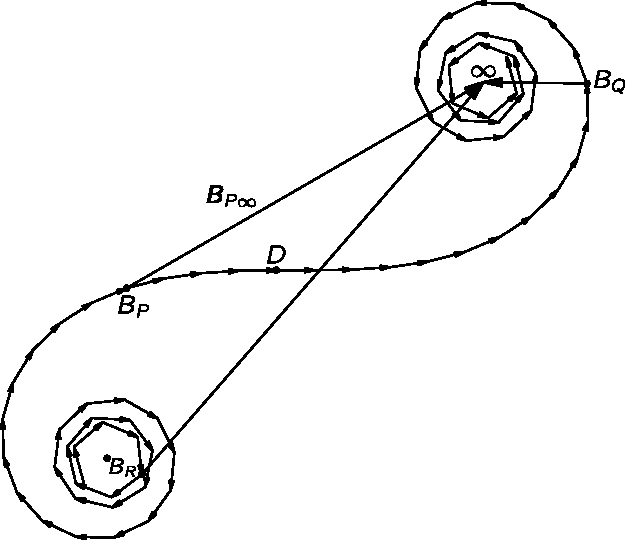
\includegraphics[width=0.8\linewidth]{fyz_fig256.pdf}
      \caption{Skládání amplitud mnoha oscilátorů kmitajících ve fázi, jejichž fázový posun se mění 
              jako druhá mocnina vzdálenosti od bodu \(D\) na předcházejícím obrázku.
               (\cite[s.~389]{Feynman01})}
      \label{fyz:fig256}
    \end{figure}
    
    Představme si tam velké množství antén, jednu těsně vedle druhé. Zajímá nás intenzita v bodě 
    \(P\). Podobá se to tomu, co jsme už dělali, ale ne zcela, neboť naše stínítko nyní není v 
    nekonečnu, Nechceme vědět, jaká je intenzita v nekonečnu, ale v konečném bodě. Při výpočtu 
    intenzity v daném místě musíme sčítat příspěvky od všech antén. Nejprve je zde anténa v bodě 
    \(D\), přesně proti bodu \(P\). Kdybychom se posunuli o málo výš, řekněme o vzdálenost \(h\), 
    časové zpoždění se zvětší. (Změní se i amplituda, neboť se změní vzdálenost, ale je to jen 
    velmi malý efekt, jsme-li od zdroje dost daleko a je mnohem méně významný než změna ve fázích.) 
    Dráhový rozdíl \(EP - DP\) je \(h^2/2s\), takže rozdíl fází se zvětšuje s druhou mocninou 
    vzdálenosti, o niž se posuneme od bodu \(D\), zatímco předtím jsme mívali \(s\) nekonečné a 
    fázový rozdíl byl \emph{přímo úměrný} \(h\). Jsou-li fáze přímo úměrné, každý vektor se sčítá 
    pootočen o konstantní úhel proti předcházejícímu. Nyní však potřebujeme křivku, jež vznikne 
    sčítáním mnoha infinitezimálně malých vektorů za podmínky, že úhel, který svírají, se 
    nezvětšuje lineárně, ale s \emph{druhou mocninou} délky křivky. Ke konstrukci takové křivky je 
    třeba trochu složitější matematiky, ale vždy jí můžeme zkonstruovat přímo nanášením vektorů a 
    měřením úhlů. V každém případě dostaneme nádhernou křivku (\emph{Cornuovo spirálu}) znázorněnou 
    na obr. \ref{fyz:fig257}. Jak ji nyní využijeme?

    \begin{figure}[ht!] %\ref{fyz:fig257}
      \centering
      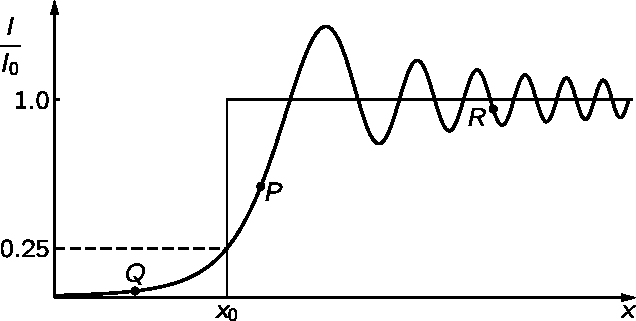
\includegraphics[width=0.7\linewidth]{fyz_fig257.pdf}
      \caption{Průběh intenzity na hranici stíu. Geometrická hranice stínu je v bodě \(x_0\).
               (\cite[s.~403]{Feynman01})}
      \label{fyz:fig257}
    \end{figure}

    Chceme-li vědět, jaká je intenzita světla například v bodě \(P\). sčítáme příspěvky, jež mají 
    různé fáze, od bodu \(D\) nahoru do nekonečna a od bodu \(D\) dolů jen po bod \(BP\)) z něhož 
    vynášíme postupně celou sérii šipek se stále se zvětšujícími úhly. Celkový příspěvek od bodu 
    \(B\) nahoru proto sleduje spirálovitou křivku. Kdyby se měla integrace v některém bodě 
    zastavit, celková amplituda by byla dána vektorem spojujícím \(B\) s tímto bodem; v tomto 
    případě jdeme až do nekonečna, takže celkový příspěvek je roven vektoru \(B\). Inflexní bod 
    \(D\) vždy odpovídá poloze bodu \(P\) a proto poloha bodu \(B\), na křivce se mění podle toho, 
    kde se bod \(P\) nachází. Proto počáteční bod výsledného vektoru bude ležet v různých místech 
    dolní levé části křivky podle toho, jak daleko nad bodem \(B\) se nachází bod \(P\). Výsledný 
    vektor \(B\) bude mít mnoho maxim a minim (obr. \ref{fyz:fig257}).
    
    
    V opačném případě, když jsme v bodě \(Q\), na opačné straně od bodu \(P\), použijeme jen jeden 
    konec spirálové křivky a ne i druhý. To znamená, že začátek se dostane jen do bodu \(B\), takže 
    výsledná intenzita osvětlení se postupně zmenšuje, jak se bod \(Q\) posunuje hlouběji do stínu.
    
    Abychom si ověřili, že jsme opravdu pochopili, můžeme ihned snadno vypočítat intenzitu světla v 
    bodě přesně proti hraně. Intenzita je zde rovna \num{1/4} intenzity dopadajícího světla. V 
    tomto případě je začátek výsledného vektoru v bodě \(D\) na obr. \ref{fyz:fig256} a z celkové 
    křivky nám zůstane jen polovina v porovnání s tím, co bychom měli, kdybychom byli hluboko v 
    osvětlené zóně. Je-li bod \(R\) hluboko v osvětlené zóně, máme celou křivku od jednoho jejího 
    konce až po druhý, tj. celý jednotkový vektor. Nacházíme-li se však na hranici stínu, máme jen 
    poloviční amplitudu, což odpovídá \num{1/4} intenzity záření.
    
    V této kapitole jsme hledali výslednou intenzitu v různých směrech od různě rozložených zdrojů. 
    V následujícím článku odvodíme vztah, který budeme potřebovat v další kapitole v teorii indexu 
    lomu. Dosud jsme vystačili s relativními intenzitami, ale tentokrát odvodíme úplný vztah pro 
    výpočet pole v konkrétní situaci.
    
  \section{Pole nábojů kmitajících v rovině}\label{fyz:IchapXXXsecVII}
    Předpokládejme, že máme mnoho zdrojů rozložených v rovině, jež současně kmitají, přičemž se 
    pohybují v rovině a mají stejnou amplitudu a stejnou fázi. Jaké bude pole v konečné, ale přitom 
    dostatečně velké vzdálenosti od roviny? (Nemůžeme se příliš přiblížit, neboť nemáme správné 
    vzorce v blízkosti zdrojů) Označíme-li rovinu nábojů \(XY\), chceme vědět, jaké pole je v bodě 
    \(P\) daleko na ose \(Z\) (obr. \ref{fyz:fig258}). Předpokládejme, že na jednotce plochy roviny 
    se nachází \(\eta\) nábojů a že každý z nich má náboj \(q\). Všechny náboje se pohybují 
    jednoduchým harmonickým pohybem se stejným směrem pohybu, amplitudou a fází. Nechť pohyb 
    každého náboje \emph{vzhledem k jeho rovnovážné poloze} je \(x_0\cos\omega t\). Pomocí 
    komplexního zápisu může být tento pohyb popsán jako \(x_0e^{i\omega t}\), přičemž máme na 
    paměti, že skutečný pohyb popisuje reálná část. 
    
    Intenzitu pole v bodě \(P\) od všech nábojů dostaneme tak, že zjistíme intenzitu od každého 
    náboje \(q\) a pak sčítáme příspěvky od všech nábojů. Víme, že radiační pole je úměrné 
    zrychlení náboje, jež je \(-\omega^2x_0e^{i\omega t}\) a je stejné pro každý náboj. Hledaná 
    intenzita elektrického pole v bodě \(P\), způsobená nábojem v bodě \(Q\), je úměrná zrychlení 
    náboje \(q\), ale musíme mít na zřeteli, že v bodě \(P\) v čase \(t\) je dáno zrychlením náboje 
    v dřívějším čase \(t' = t - r/c\), kde \(r/c\) je čas, který potřebují vlny pole, aby prošly 
    vzdálenost \(r\) od \(Q\) do \(P\). Proto je pole v bodě \(P\) úměrné
    \begin{equation}\label{fyz:eq327}
      - \omega^2x_0e^{i\omega(t-r/c)}.
    \end{equation}
    
    \begin{figure}[ht!] %\ref{fyz:fig258}
      \centering
      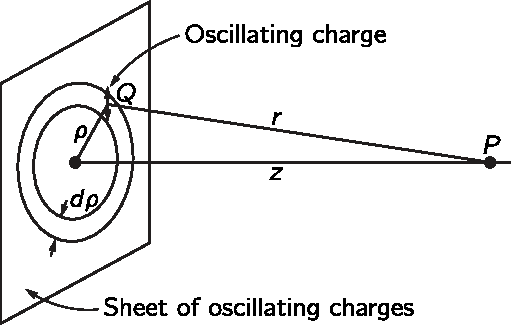
\includegraphics[width=0.8\linewidth]{fyz_fig258.pdf}
      \caption{Radiační pole nábojů oscilujících v rovině
               (\cite[s.~404]{Feynman01})}
      \label{fyz:fig258}
    \end{figure}
    
    Dosadíme-li toto zrychlení do našeho vztahu pro intenzitu elektrického pole ve velkých  
    vzdálenostech od vyzařujícího náboje, dostaneme inteznitu pole v \(P\) od náboje v 
    \begin{equation*}
      \left(\begin{matrix}
         \text{Intenzita pole v P}  \\
         \text{od náboje v Q}
      \end{matrix}\right) \approx 
      \frac{q}{4\pi\varepsilon_0c^2}
      \frac{\omega^2x_0e^{i\omega(t-r/c)}}{r}\text{ (přibližně)}.
    \end{equation*}
    
    Tento vztah není zcela přesný, neboť jsme neměli použít zrychlení náboje, ale jeho 
    \emph{složku} kolmou na přímku \(QP\). Budeme však předpokládat, že bod \(P\) je tak daleko v 
    porovnání se vzdáleností bodu \(Q\) od osy (vzdálenost \(\varrho\) na obr. \ref{fyz:fig258}), 
    že při změnách, jež budeme brát v úvahu, můžeme kosinový faktor (jenž by byli tak roven 
    přibližně \num{1}) vynechat.
    
    Abychom dostali celkovou intenzitu pole v \(P\), sčítáme vlivy od všech nábojů, jež jsou v 
    rovině. Samozřejmě, měli bychom udělat vektorový součet, ale protože směr intenzity pole je 
    téměř stejný pro všechny náboje, můžeme, v rámci již uvedené aproximace, prostě sčítat 
    velikosti intenzit. V naší aproximaci závisí intenzita pole v bodě \(P\) jen na vzdálenosti 
    \(r\), takže všechny náboje vzdálené o stejné \(r\) vytvářejí stejná pole. Proto nejdříve 
    sčítáme pole od nábojů rozložených na prstenci šířky \(\dd{\varrho}\) s poloměrem \(\varrho\). 
    Potom integrací přes všechna \(\varrho\) dostaneme celkové pole.
    
    Počet nábojů na prstenci se rovná součinu velikosti plochy prstence \(2\pi\varrho\dd{\varrho}\) 
    počtu nábojů na jednotkové ploše \(\eta\). Takže máme výsledné pole v bodě \(P\)
    \begin{equation}\label{fyz:eq333}
      \int\frac{q}{4\pi\varepsilon_0c^2}
      \frac{\omega^2x_0e^{i\omega(t-r/c)}}{r}
      \cdot\eta2\pi\varrho\dd{\varrho}.
    \end{equation}
    
    Tento integrál chceme vypočítat pro \(\varrho\) od \(\varrho = 0\) do \(\varrho = \infty\). 
    Proměnná \(t\) je po dobu integrace konstantní, takže proměnnými veličinami jsou jen 
    \(\varrho\) a \(r\). Vynecháme-li na chvíli všechny konstantní faktory, včetně faktoru 
    \(e^{i\omega t}\), žádaný integrál má tvar
    \begin{equation}\label{fyz:eq328}
      \int_{\varrho=0}^{\varrho=\infty}\frac{e^{-i\omega(r/c)}}{r}\varrho\dd{\varrho}.
    \end{equation}
    Kjeho výpočtu potřebujeme použít vztah mezi \(r\) a \(\varrho\) 
    \begin{equation}\label{fyz:eq329}
      r^2 = \varrho^2 + z^2.
    \end{equation}
    Protože \(z\) nezávisí na \(\varrho\), diferencováním máme 
    \begin{equation*}
      2r\dd{r} = 2\varrho\dd{\varrho},
    \end{equation*}
    což je výhodné, neboť v integrálu můžeme zaměnit \(\varrho\dd{\varrho}\) za \(r\dd{r}\) a \(r\) 
    se vyruší s \(r\) ve jmenovateli. Hledaný integrál má pak jednodušší tvar
    \begin{equation}\label{fyz:eq330}
      \int_{r=0}^{r=z}e^{-i\omega(r/c)}\dd{r}.
    \end{equation}
    Integrace exponenciální funkce je velmi snadná. Funkci dělíme koeficientem, jenž je v exponentu 
    u \(r\) a exponenciálu vyčíslíme v integračních mezích; ale integrační meze pro \(r\) nejsou 
    stejné jako pro \(\varrho\). Pro \(\varrho = 0\) máme \(r = z\), takže integrujeme pro \(r\) od 
    \(z\) do nekonečna. Dostáváme výsledek
    \begin{equation}\label{fyz:eq331}
      -\frac{c}{i\omega}\left[e^{-i\infty} - e^{-(i\omega/c)z}\right],
    \end{equation}
    kde za \(\omega r/c\) v nekonečnu jsme napsali \(\infty\), neboť oba zápisy označují velmi 
    velké číslo!
    
    Přitom \(e^{-i\infty}\) je záhadná veličina. Její reálná část je například rovna 
    \(\cos(-\infty)\), co je matematicky řečeno, úplně neurčitá veličina (i když bychom očekávali, 
    že to bude hodnota někde nebo všude mezi \num{+1} a \num{-1}!) Ve \emph{fyzikální} situaci to 
    však může označovat něco docela rozumného a obvykle to lze považovat za nulu. Abychom si 
    ozřejmili, že je to tak i v našem případě, vraťme se k původnímu integrálu (\ref{fyz:eq330}).
    
    \begin{figure}[ht!] %\ref{fyz:fig259}
      \centering
      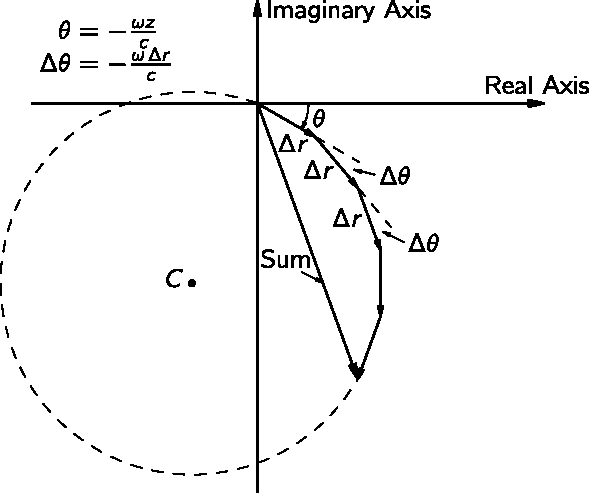
\includegraphics[width=0.8\linewidth]{fyz_fig259.pdf}
      \caption{Grafické řešení integrálu \(\int_z^\infty e^{-i\omega r/c}\dd{r}\)
               (\cite[s.~406]{Feynman01})}
      \label{fyz:fig259}
    \end{figure}
    
    Integrál (\ref{fyz:eq330}) můžeme chápat jako součet mnoha malých komplexních čísel, přičemž 
    každé má v komplexní rovině velikost \(\Delta r\) a směrový úhel \(\varphi = - \omega r/c\). 
    Tento součet se můžeme pokusit vypočítat graficky. Na obr. \ref{fyz:fig259} máme nakreslených 
    prvních pět členů součtu. Každý úsek má délku \(\Delta r\) a s předcházejícím svírá úhel 
    \(\Delta\varphi = -= - \omega\Delta r/c\). Součet těchto prvních pěti členů je znázorněn šipkou 
    od počátku ke konci pátého úseku. Přidáváním dalších členů bychom sledovali mnohoúhelník, až 
    bychom se dostali nazpět do počátku (přibližně) a začali opět dokola. Přidáváním dalších členů 
    bychom se točili stále dokola v blízkosti kružnice, o níž lze snadno ukázat, že její poloměr je 
    roven \(c/\omega\). Vidíme, proč integrál nedává určitou hodnotu. 
    
    Nyní se však musíme vrátit zpět k fyzice, jaká je v naší situaci. V žádné reálné situaci nemůže 
    být rovina nábojů nekonečně rozsáhlá, ale musí někde končit. Kdyby končila najednou a měla 
    přesně kruhový tvar, náš integrál by měl nějakou hodnotu na kružnici na obr. \ref{fyz:fig259}. 
    Připustíme-li, aby počet nábojů v rovině postupně klesal v nějaké velké vzdálenosti od středu 
    (nebo končil náhle, ale nepravidelně, takže pro velké \(\varrho\) nebude přispívat celý 
    prstenec šířky \(\dd{\varrho}\)), koeficient bude v přesném integrálu klesat k nule. Vzhledem k 
    tomu, že budeme sčítat klesající členy, ale stále se odchylující o stejný úhel, grafem našeho 
    integrálu bude křivka ve tvaru spirály, Spirála nakonec skončí ve středu našeho původního 
    kruhu, jak je to nakresleno na obr. \ref{fyz:fig260}. \emph{Fyzikálně} správný integrál dává 
    komplexní číslo\( A\) znázorněné na obrázku šipkou od počátku do středu kruhu, což je právě 
    rovno
    \begin{equation}\label{fyz:eq332}
      \frac{c}{i\omega}e^{-i\omega z/c},
    \end{equation}
    jak se můžeme sami přesvědčit. Stejný výsledek bychom dostali z rovnice (\ref{fyz:eq331}), 
    kdybychom položili \(e^{-i\infty} = 0\). (Je zde ještě další důvod, proč se příspěvek k 
    integrálu pro velké hodnoty \(r\) zmenšuje; musíme totiž brát projekci vektoru zrychlení do 
    roviny kolmé na spojnici \(PQ\), což jsme zanedbávali.)
    
    \begin{figure}[ht!] %\ref{fyz:fig260}
      \centering
      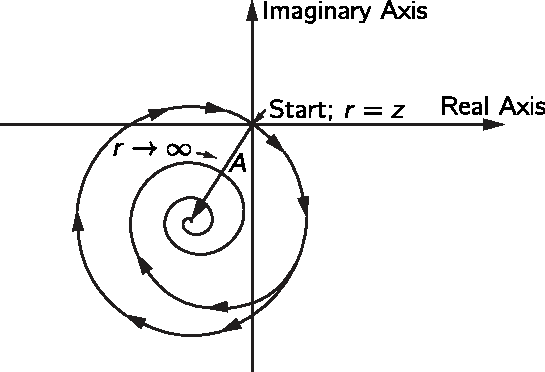
\includegraphics[width=0.8\linewidth]{fyz_fig260.pdf}
      \caption{Grafické řešení integrálu \(\int_z^\infty\eta e^{-i\omega r/c}\dd{r}\)
               (\cite[s.~406]{Feynman01})}
      \label{fyz:fig260}
    \end{figure}
    
    Nás zajímají jen fyzikálně reálné situace, proto zvolíme \(e^{-i\infty} = 0\) rovno nule. 
    Vrátíme-li se ke vztahu pro výsledné pole (\ref{fyz:eq333}) se všemi činiteli, jež jsou v 
    integrálu, máme výsledné pole v \(P\)
    \begin{equation}\label{fyz:eq334}
      -\frac{\eta q}{2\varepsilon_0c}i\omega x_0e^{-i\omega(t - z/c)},
    \end{equation}
    (mějme na zřeteli, že \(1/i = -i\)). Je zajímavé si všimnout, že (\(i\omega x_0e^{-i\omega 
    t}\)) je rovnoprávě rychlosti pohybu nábojů, takže rovnici pro výpočet výsledného pole v \(P\) 
    můžeme napsat také jako
    \begin{equation}\label{fyz:eq335}
      -\frac{\eta q}{2\varepsilon_0c}(\text{rychlost nábojů v čase }t - z/c).
    \end{equation}
    Je to trochu překvapující, protože časové zpoždění je dáno právě vzdáleností \(z\), což je 
    nejkratší vzdálenost od \(P\) do roviny nábojů. Ale naštěstí vychází právě takový jednoduchý 
    výsledek. (Mimochodem můžeme dodat, že i když bylo naše odvození platné jen pro dostatečně 
    velké vzdálenosti od roviny oscilujících nábojů, ukazuje se, že vztah (\ref{fyz:eq334}) nebo 
    (\ref{fyz:eq335}) platí pro libovolnou vzdálenost \(z\), dokonce i pro \(z<\lambda\)).
    
  \section{Příklady a cvičení}\label{fyz:IchapXXXsecVIII}


%} %tikzset
%---------------------------------------------------------------------------------------------------
\printbibliography[title={Seznam literatury}, heading=subbibliography]
\addcontentsline{toc}{section}{Seznam literatury}